\documentclass[hidelinks,12pt]{article}
\usepackage[left=0.25cm,top=1cm,right=0.25cm,bottom=1cm]{geometry}
%\usepackage[landscape]{geometry}
\textwidth = 20cm
\hoffset = -1cm
\usepackage[utf8]{inputenc}
\usepackage[spanish,es-tabla]{babel}
\usepackage[autostyle,spanish=mexican]{csquotes}
\usepackage[tbtags]{amsmath}
\usepackage{nccmath}
\usepackage{amsthm}
\usepackage{amssymb}
\usepackage{mathrsfs}
\usepackage{graphicx}
\usepackage{subfig}
\usepackage{standalone}
\usepackage[outdir=./Imagenes/]{epstopdf}
\usepackage{siunitx}
\usepackage{physics}
\usepackage{color}
\usepackage{float}
\usepackage{hyperref}
\usepackage{multicol}
%\usepackage{milista}
\usepackage{anyfontsize}
\usepackage{anysize}
%\usepackage{enumerate}
\usepackage[shortlabels]{enumitem}
\usepackage{capt-of}
\usepackage{bm}
\usepackage{relsize}
\usepackage{placeins}
\usepackage{empheq}
\usepackage{cancel}
\usepackage{wrapfig}
\usepackage[flushleft]{threeparttable}
\usepackage{makecell}
\usepackage{fancyhdr}
\usepackage{tikz}
\usepackage{bigints}
\usepackage{scalerel}
\usepackage{pgfplots}
\usepackage{pdflscape}
\pgfplotsset{compat=1.16}
\spanishdecimal{.}
\renewcommand{\baselinestretch}{1.5} 
\renewcommand\labelenumii{\theenumi.{\arabic{enumii}})}
\newcommand{\ptilde}[1]{\ensuremath{{#1}^{\prime}}}
\newcommand{\stilde}[1]{\ensuremath{{#1}^{\prime \prime}}}
\newcommand{\ttilde}[1]{\ensuremath{{#1}^{\prime \prime \prime}}}
\newcommand{\ntilde}[2]{\ensuremath{{#1}^{(#2)}}}

\newtheorem{defi}{{\it Definición}}[section]
\newtheorem{teo}{{\it Teorema}}[section]
\newtheorem{ejemplo}{{\it Ejemplo}}[section]
\newtheorem{propiedad}{{\it Propiedad}}[section]
\newtheorem{lema}{{\it Lema}}[section]
\newtheorem{cor}{Corolario}
\newtheorem{ejer}{Ejercicio}[section]

\newlist{milista}{enumerate}{2}
\setlist[milista,1]{label=\arabic*)}
\setlist[milista,2]{label=\arabic{milistai}.\arabic*)}
\newlength{\depthofsumsign}
\setlength{\depthofsumsign}{\depthof{$\sum$}}
\newcommand{\nsum}[1][1.4]{% only for \displaystyle
    \mathop{%
        \raisebox
            {-#1\depthofsumsign+1\depthofsumsign}
            {\scalebox
                {#1}
                {$\displaystyle\sum$}%
            }
    }
}
\def\scaleint#1{\vcenter{\hbox{\scaleto[3ex]{\displaystyle\int}{#1}}}}
\def\bs{\mkern-12mu}


\title{1 - Coordenadas curvilíneas ortogonales \\[0.3em]  \large{Matemáticas Avanzadas de la Física}\vspace{-3ex}}
\author{M. en C. Gustavo Contreras Mayén}
\date{ }
\begin{document}
\vspace{-4cm}
\maketitle
\fontsize{14}{14}\selectfont
\tableofcontents
\newpage

\section{Coordenadas curvilíneas ortogonales.}
\subsection{Introducción.}

En el espacio euclidiano tridimensional las coordenadas cartesianas se definen en términos de tres familias de planos perpendiculares:
\begin{align*}
x = x_{0}, \hspace{0.25cm} y = y_{0}, \hspace{0.25cm} z = z_{0}
\end{align*}
Como vemos en la figura \ref{fig:figura_planos_cartesianos}:
\begin{figure}[H]
   \centering
   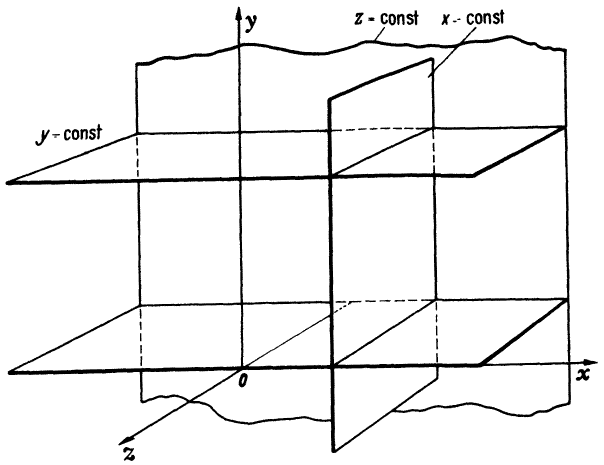
\includegraphics[scale=1.5]{Imagenes/Planos_Coordenadas_Cartesianas.png}
   \caption{Las superficies coordenadas son los planos $x=\mbox{cte.}, y=\mbox{cte.}, z=\mbox{cte.}$}
   \label{fig:figura_planos_cartesianos}
\end{figure}
La intersección de los planos $x = x_{0}$ y $y = y_{0}$ genera una línea recta paralela al eje $z$
que pasa por el punto $(x_{0}, y_{0}, 0)$.
\par
La intersección de los tres planos $x = x_{0}, y = y_{0}, z = z_{0}$ genera un punto de coordenadas $(x_{0}, y_{0}, z_{0})$.

\subsubsection*{Coordenadas esféricas.}

Las coordenadas esféricas se definen en términos de tres superficies: esferas concéntricas, conos con el mismo vértice y planos meridianos.
\par
Un punto tiene coordenadas $(r, \theta, \phi)$ y las tres superficies son perpendiculares en cada punto.
\begin{figure}[H]
   \centering
   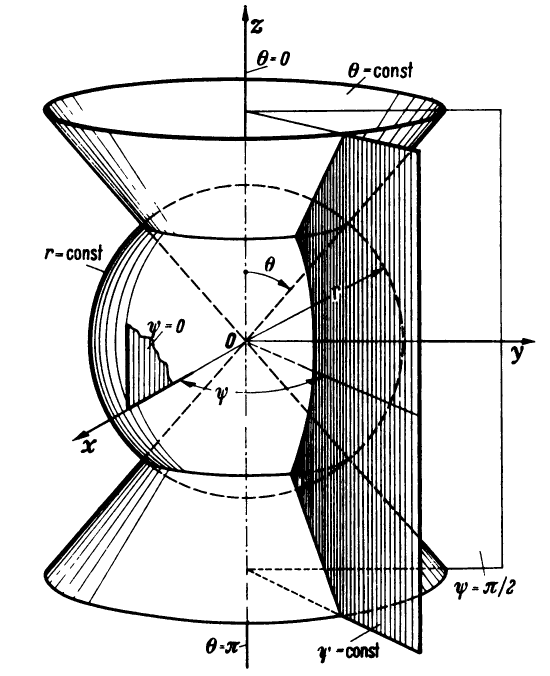
\includegraphics[scale=1.5]{Imagenes/Planos_Coordenadas_Esfericas.png}
   \caption{Coordenadas esféricas $(r, \theta, \phi)$. Las superficies coordenadas son \emph{esferas} ($r = \mbox{cte.}$), \emph{conos circulares} $(\theta = \mbox{const})$, \emph{planos meridianos} $(\phi = \mbox{cte.})$}
   \label{fig:figura_planos_esfericos}
\end{figure}
La intersección del cono y la esfera genera una circunferencia a lo largo de la cual varía sólo la coordenada $\phi$.
\par
La intersección de la esfera y el plano meridiano genera un arco de meridiano a lo largo del cual sólo $\theta$ varía, y la intersección del cono y el plano genera una recta radial a lo largo de la cual sólo $r$ varía.
\par
La conexión entre coordenadas cartesianas y esféricas (regla de transformación) tiene la forma:
\begin{align*}
x &= r \, \sin \theta \cos \varphi \\
y &= r \sin \theta \sin \varphi \\
z &= r \cos \theta
\end{align*}

\subsubsection*{Coordenadas cilíndricas.}

De manera análoga tenemos que para las coordenadas cilíndricas, se construyen con tres superficies perpendiculares: cilindros concéntricos, planos meridianos y planos horizontales, como se ve en la figura \ref{fig:figura_planos_cilindricos}.
\par
A cada una se le asocian, las coordenadas $(\rho, \phi, z)$ respectivamente.
\begin{figure}[H]
   \centering
   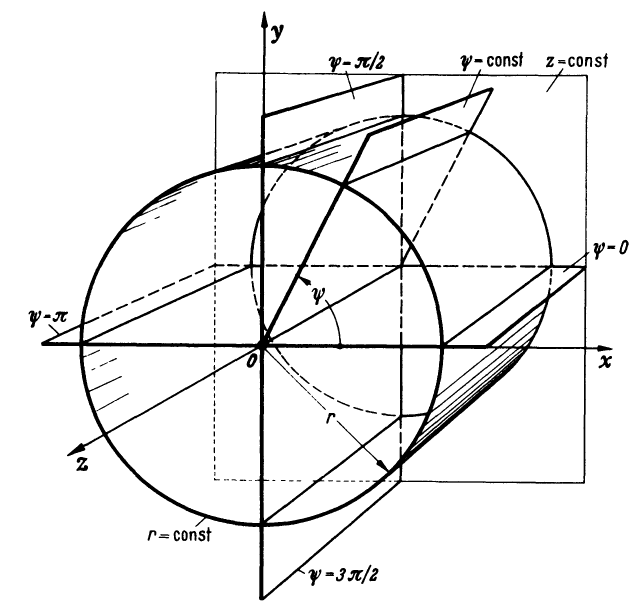
\includegraphics[scale=1.5]{Imagenes/Planos_Coordenadas_Cilindricas.png}
   \caption{Coordenadas cilíndricas $(\rho, \theta, z)$. Las superficies coordenadas son \emph{cilindros circulares} ($\rho = \mbox{cte.}$), \emph{planos meridianos} $(\theta = \mbox{const})$ que intersectan al eje $x$, \emph{planos paralelos} $(z = \mbox{cte.})$}
   \label{fig:figura_planos_cilindricos}
\end{figure}
Las reglas de transformación entre coordenadas cartesianas y cilíndricas son de la forma:
\begin{align*}
x &= \rho \, \cos \phi \\ 
y &= \rho \, \sin \phi \\
z &= z
\end{align*}

%Ref. Sepúlveda (2004) - Lecciones de Física Matemática. 1. Coord. Curvilíneas ortogonales.

\subsection{Coordenadas curvilíneas ortogonales.}

Una generalización directa permite pensar en tres familias de superficies, en general curvas, que en cada punto del espacio se intersectan en ángulo recto.
\par
Estas superficies pueden describirse mediante las ecuaciones:
\begin{align*}
u_{1} &= f_{1}(x, y, z) \\
u_{2} &= f_{2}(x, y, z) \\
u_{3} &= f_{3}(x, y, z)
\end{align*}
De manera equivalente:
\begin{align*}
x &= x(u_{i}) \\
y &= y(u_{i}) \\
z &= z(u_{i})
\end{align*}
Estas ecuaciones son a la vez las reglas de transformación entre \emph{coordenadas cartesianas} y las \emph{coordenadas curvilíneas ortogonales}.
\par
Las superficies $u_{1} = \mbox{cte.}$ y $u_{2} = \mbox{cte.}$ se intersectan en una curva a lo largo de la cual solo $u_{3}$ varía, esta curva define a la coordenada $u_{3}$, como se ve en la figura \ref{fig:figura_Sistema_Curvilineo_Ortogonal}.
\begin{figure}[H]
   \centering
   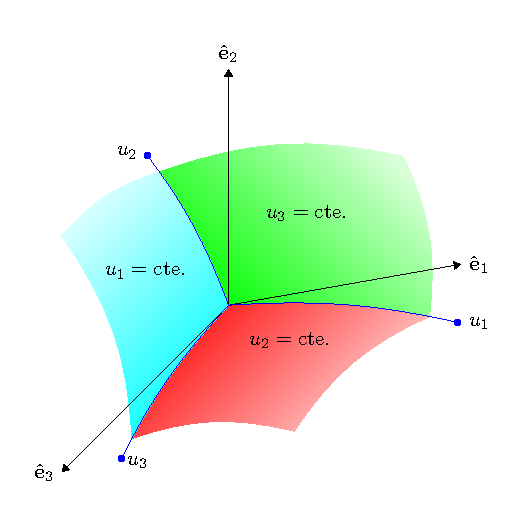
\includegraphics[scale=1]{Imagenes/Sistema_Curvilineo_Ortogonal.eps}
   \caption{Sistema curvilíneo ortogonal. Los vectores unitarios $(\vu{e}_{1}, \vu{e}_{2}, \vu{e}_{3})$ son tangentes a las superficies.}
   \label{fig:figura_Sistema_Curvilineo_Ortogonal}
\end{figure}
Análogamente las superficies $u_{1} = \mbox{cte.}$ y $u_{3} = \mbox{cte.}$ generan la curva $u_{2}$; y las superficies $u_{2} = \mbox{cte.}$ y $u_{3} = \mbox{cte.}$ generan la curva $u_{1}$.
\par   
La intersección de las tres superficies genera un punto cuyas coordenadas son $(u_{1}, u_{2}, u_{3})$. Dado un punto $(x, y, z)$ es posible asignarle unívocamente un conjunto $(u_{1}, u_{2}, u_{3})$ de coordenadas curvilíneas.
\par
El sistema de coordenadas curvilíneas construido con estas superficies, tiene las siguientes características:
\begin{enumerate}
\item Los ejes coordenados son en general curvas que se intersectan en ángulo recto, de modo que los vectores unitarios $\left\{ \vu{e}_{i} \right\}$, que son tangentes a las curvas, generan una base ortonormal tridimensional.
\item La orientación de la base $\left\{ \vu{e}_{i} \right\}$ puede cambiar de punto a punto, preservándose su ortonormalidad.
\item El significado físico de los diferenciales de las coordenadas \emph{no es necesariamente una longitud}. En coordenadas esféricas, tenemos una longitud y dos ángulos.
\end{enumerate}
En el curso nos enfocaremos en el estudio de este tipo de sistemas: coordenados ortogonales, los sistemas coordenados no ortogonales no los revisaremos.

\subsection*{Campo escalar.}

Un \emph{campo escalar} se define dando un valor numérico en cada punto del espacio.
\par
El valor de una cantidad escalar en un punto definido del espacio es independiente del sistema de coordenadas que se utilice.
\par
Por lo que decimos que si $(x, y, z)$, $(\rho, \phi, z)$, $(r, \theta, \phi)$ denotan el mismo punto del espacio físico, el valor que en ese punto tome, por ejemplo, la presión atmosférica es el mismo.

\subsection*{Campo vectorial.}

Los campos vectoriales se definen dando en cada punto del espacio el valor de tres cantidades, conocidas como las \emph{componentes vectoriales}.
\par
Aunque los vectores unitarios y los valores de cada componente sean diferentes en cada sistema de coordenadas, es sin embargo cierto que el vector $\vb{A}$ no cambia cuando cambiamos de sistema coordenado.
\par
Por lo que podemos decir que si los vectores unitarios $\vu{e}_{i}$ y $\vu{e}_{i}^{\prime}$, y las componentes $A_{i}$ y $\ptilde{A}_{i}$ en dos sistemas coordenados $S$ y $\ptilde{S}$, entonces:
\begin{align*}
\vb{A} = \nsum_{i=1}^{3} A_{i} \, \vu{e}_{i} = \nsum_{i=1}^{3} \ptilde{A}_{i} \, \vu{e}_{i}^{\prime}
\end{align*}
Esto significa que un vector es \emph{invariante} bajo transformaciones de coordenadas.
\par
Los campos escalares son también invariantes bajo transformaciones de coordenadas. En la \emph{teoría de transformación} se revisa estos temas.

\subsection*{Ecuaciones matemáticas.}

De esta manera es posible escribir ecuaciones cuya forma matemática es la misma en todos los sistemas de coordenadas en el espacio $\mathbb{R}^{3}$ euclidiano.
\par
Por ejemplo, la ecuación de onda:
\begin{align*}
\laplacian{\psi} - \dfrac{1}{v^{2}} \pdv[2]{\psi}{t} = 0
\end{align*}
es válida en todos los sistemas coordenados, es decir, es invariante bajo transformación de coordenadas.

\section{Teoría de transformación.}

En el espacio euclidiano es siempre posible construir un sistema coordenado cartesiano que se extienda indefinidamente.
\par
A partir de él podemos generar múltiples sistemas coordenados, mediante el uso de las superficies $u_{i} = f(x, y, z)$
\par
Dado que de manera recíproca, $(x, y, z)$ son funciones de $u_{i}$, es decir:
\begin{align*}
x &= x(u_{i}) \\
y &= y(u_{i}) \\
z &= z(u_{i})
\end{align*}
Entonces podemos escribir:
\begin{align*}
\dd{x} = \pdv{x}{u_{1}} \dd{u_{1}} + \pdv{x}{u_{2}} \dd{u_{2}} + \pdv{x}{u_{3}} \dd{u_{3}} \\[0.5em]
\dd{y} = \pdv{y}{u_{1}} \dd{u_{1}} + \pdv{y}{u_{2}} \dd{u_{2}} + \pdv{y}{u_{3}} \dd{u_{3}} \\[0.5em]
\dd{z} = \pdv{z}{u_{1}} \dd{u_{1}} + \pdv{z}{u_{2}} \dd{u_{2}} + \pdv{z}{u_{3}} \dd{u_{3}}
\end{align*}
Estas tres ecuaciones son las componentes de la ecuación vectorial\footnote{Con la finalidad de simplificar la notación, los vectores se indicarán en \textbf{negritas}, el colocar una flecha encima en ocasiones dificulta la lectura, por lo que en general se ocupará esta notación tipográfica para diferenciarlo de una componente.}:
\begin{align}
\begin{aligned}
\dd{\vb{r}} &= \pdv{\vb{r}}{u_{1}} \dd{u_{1}} + \pdv{\vb{r}}{u_{2}} \dd{u_{2}} + \pdv{\vb{r}}{u_{3}} \dd{u_{3}} = \\[0.5em]
&= \nsum_{i=1}^{3} \pdv{\vb{r}}{u_{i}} \dd{u_{i}}
\end{aligned}
\label{eq:ecuacion_01_01}
\end{align}
En general, el factor $\pdv*{\vb{r}}{u_{i}}$ en la ec. (\ref{eq:ecuacion_01_01}) es un vector \emph{no unitario} que toma en cuenta la variación de $\vb{r}$ solo en la dirección de $u_{i}$, y es por tanto, tangente a la curva coordenada $u_{i}$.
\par
Con el fin de introducir una \emph{base normalizada} $\vu{e}_{i}$, es decir, un conjunto de vectores unitarios, escribimos:
\begin{align}
\pdv{\vb{r}}{u_{i}} = h_{i} \, \vu{e}_{i}
\label{eq:ecuacion_01_02}
\end{align}
donde $\abs{\vb{e}_{i}} = 1$ y $h_{i}$ son funciones de $u_{i}$, que llamaremos \emph{\textcolor{blue}{factores de escala}}.
\par
Se sigue entonces que el diferencial de desplazamiento es:
\begin{align*}
\dd{\vb{r}} = \nsum_{i=1}^{3} h_{i} \, \vu{e}_{i} \dd{u_{i}}
\end{align*}
\par
Como hicimos la aclaración de trabajar con bases \emph{ortonormales} (perpendiculares y unitarias), podemos escribir:
\begin{align}
\vu{e}_{i} \cdot \vu{e}_{j} = \delta_{ij}
\label{eq:ecuacion_01_03}
\end{align}
donde $\delta_{ij}$ es la delta de Kronecker:
\begin{align*}
\delta_{ij} = 
\begin{cases}
0 & \mbox{si } i \neq j \\
1 & \mbox{si } i = j
\end{cases}
\end{align*}
Entonces tendremos que:
\begin{align*}
\vu{e}_{1} \cdot \vu{e}_{2} = \vu{e}_{2} \cdot \vu{e}_{3} = \vu{e}_{3} \cdot \vu{e}_{1} = 0  
\end{align*}
y además:
\begin{align*}
\vu{e}_{1} \cdot \vu{e}_{1} = \abs{\vu{e}_{1}}^{2} = \abs{\vu{e}_{2}}^{2} = \abs{\vu{e}_{3}}^{2} = 1
\end{align*}
Por la ecuación (\ref{eq:ecuacion_01_02}), los factores de escala se definen por:
\begin{align}
\abs{\pdv{\vb{r}}{u_{i}}} = h_{i}
\label{eq:ecuacion_01_04}
\end{align}
por lo que es fácil calcular los factores de escala.
\par
En consecuencia los vectores unitarios en coordenadas curvilíneas (ec. \ref{eq:ecuacion_01_02}) se escriben como:
\begin{align}
\vu{e}_{i} = \dfrac{1}{h_{i}} \, \pdv{\vb{r}}{u_{i}}
\label{eq:ecuacion_01_05}
\end{align}

\subsection*{Ejemplo}

Como ejemplo haremos el cambio de coordenadas cartesianas a coordenadas esféricas.
\begin{align*}
(x, y, z) \longrightarrow (r, \theta, \varphi)
\end{align*}
Un punto $P$ puede localizarse mediante las coordenadas cartesianas $(x, y, z)$ y también mediante coordenadas esféricas $(r, \theta, \varphi)$, donde:
\\[0.5em]
\begin{minipage}{0.4\linewidth}
\begin{align*}
-\infty \le x \le \infty \\
-\infty \le y \le \infty \\
-\infty \le z \le \infty
\end{align*}
\end{minipage}
\hspace{2cm}
\begin{minipage}{0.4\linewidth}
\begin{align*}
r \geq 0 \\
0 \le \theta \le \pi \\
0 \le \varphi \le 2 \, \pi
\end{align*}
\end{minipage}
\\[0.5em]
Donde:
\begin{itemize}
\item $r = \abs{\vb{r}}$ es la coordenada radial.
\item $\theta$ es la coordenada polar.
\item $\varphi$ es la coordenada azimutal.
\end{itemize}

De la figura (\ref{fig:figura_planos_esfericos}) la \enquote{conexión} (regla de transformación)  entre las coordenadas cartesianas y esféricas es:
\begin{align*}
x &= r \, \sin \theta \, \cos \varphi \\
y &= r \, \sin \theta \, \sin \varphi \\
z &= r \, \cos \theta
\end{align*}
\begin{align*}
r &= \sqrt{x^{2} + y^{2} + z^{2}} \\
\theta &= \cos^{-1} \left( z / \sqrt{x^{2} + y^{2} + z^{2}} \right) \\
\varphi &= \tan^{-1} (y/x)
\end{align*}

Entonces el vector de posición es:
\begin{align}
\begin{aligned}
\vb{r} &= \vu{i} \, x + \vu{j} \, y + \vu{k} \, z \\
&= \vu{i} \, r \, \sin \theta \, \cos \varphi + \vu{j} \, r \, \sin \theta \, \sin \varphi + \vu{k} \, r \cos \theta 
\end{aligned}
\label{eq:ecuacion_01_06}
\end{align}

Por lo que podemos calcular los $\pdv*{\vb{r}}{u_{i}}$. Entonces tenemos que:
\begin{align*}
\pdv{\vb{r}}{r} = \vu{i} \, \sin \theta \, \cos \varphi + \vu{j} \, \sin \theta \, \sin \varphi + \vu{k} \, \cos \theta
\end{align*}
Así al calcular la norma:
\begin{align*}
\abs{\pdv{\vb{u}}{r}} &= \sqrt{\sin^{2} \theta \, \cos^{2} \varphi + \sin^{2} \theta \, \sin^{2} \varphi + \cos^{2} \theta} \\[0.5em]
&= 1
\end{align*}

Entonces por la ec. (\ref{eq:ecuacion_01_04}):
\begin{align*}
\abs{\pdv{\vb{r}}{u_{i}}} = h_{i}
\end{align*}
Tendremos el primer factor de escala:
\begin{align*}
h_{1} = h_{r} = 1
\end{align*}

El segundo factor $\pdv*{\vb{r}}{\theta}$ es:
\begin{align*}
\pdv{\vb{r}}{\theta} = \vu{i} \, r \, \cos \theta \, \cos \varphi + \vu{j} \, r \, \cos \theta \, \sin \varphi - \vu{k} \, r \, \sin \theta
\end{align*}
\par
Entonces:
\begin{align*}
\abs{\pdv{\vb{u}}{\theta}} &= \sqrt{r^{2} (\cos^{2} \theta \, \cos^{2} \varphi + \cos^{2} \theta \, \sin^{2} \varphi + \sin^{2} \theta)} \\[0.5em]
&= r
\end{align*}
\par
Así: $h_{2} = h_{\theta} = r$
\par
Para el siguiente factor de escala:
\begin{align*}
\pdv{\vb{r}}{\varphi} = - \vu{i} \, r \, \sin \theta \, \sin \varphi + \vu{j} \, r \, \sin \theta \, \cos \varphi
\end{align*}
\par
Entonces:
\begin{align*}
\abs{\pdv{\vb{u}}{\varphi}} &= \sqrt{r^{2} (\sin^{2} \theta \, \sin^{2} \varphi + \sin^{2} \theta \, \cos^{2} \varphi)} \\[0.5em]
&= r \, \sin \theta
\end{align*}
\par
Así: $h_{3} = h_{\varphi} = r \, \sin \theta$
\par
Entonces los factores de escala para el sistema coordenado esférico son:
\begin{align}
\begin{aligned}
h_{r} &= 1 \\[0.5em]
h_{\theta} &= r \\[0.5em]
h_{\varphi} &= r \, \sin \theta
\end{aligned}
\label{eq:ecuacion_01_07}
\end{align}
\par
Al reemplazar los factores de escala en la ec. (\ref{eq:ecuacion_01_05}), los vectores unitarios en coordenadas esféricas pueden expresarse en términos de coordenadas cartesianas, como:
\begin{align}
\begin{aligned}
\vu{e}_{r} &= \vu{i} \, \sin \theta \, \cos \varphi + \vu{j} \, \sin \theta \, \sin \varphi + \vu{k} \, \cos \theta \\[0.25em]
\vu{e}_{\theta} &= \vu{i} \, \cos \theta \, \cos \varphi + \vu{j} \, \cos \theta \, \sin \varphi - \vu{k} \, \sin \theta \\[0.25em]
\vu{e}_{\varphi} &= - \vu{i} \, \sin \varphi + \vu{j} \, \cos \varphi
\end{aligned}
\label{eq:ecuacion_01_08}
\end{align}
Donde: $(\vu{e}_{1}, \vu{e}_{2}, \vu{e}_{3}) = (\vu{e}_{r}, \vu{e}_{\theta}, \vu{e}_{\varphi})$
\par
Las ecs. (\ref{eq:ecuacion_01_08}) pueden invertirse algebraicamente para expresar los vectores unitarios $\vu{i}, \vu{j}, \vu{k}$ en términos de $\vu{e}_{r}, \vu{e}_{\theta}, \vu{e}_{\varphi}$, tal que:

\begin{align*}
\vu{i} &= \vu{e}_{r} \, \sin \theta \, \cos \varphi + \vu{e}_{\theta} \, \cos \theta \, \cos \varphi - \vu{e}_{\varphi} \, \sin \varphi \\[0.5em]
\vu{j} &= \vu{e}_{r} \, \sin \theta \, \sin \varphi + \vu{e}_{\theta} \, \cos \theta \, \sin \varphi + \vu{e}_{\varphi} \, \cos \varphi \\[0.5em]
\vu{k} &= \vu{e}_{r} \, \cos \theta - \vu{e}_{\theta} \, \sin \theta
\end{align*}
% \par
% \noindent
% \textbf{Ejercicio a cuenta (1).}
% \\
% Considera la transformación de coordenadas:
% \begin{align*}
% x &= 2 \, u \, v \\[0.5em]
% y &= u^{2} - v^{2} \\[0.5em]
% z &= w
% \end{align*}
% Demuestra que el nuevo sistema de coordenadas es ortogonal.

\section{Derivadas de vectores unitarios.}

En aplicaciones de análisis vectorial se requiere utilizar las derivadas parciales $\pdv*{\vu{e}_{i}}{u_{j}}$
\par
Partiendo de:
\begin{align*}
\dd{\vb{r}} = \nsum_{i} h_{i} \, \vu{e}_{i} \dd{u_{i}}
\end{align*}
\par
Entonces podemos escribir:
\begin{align*}
\pdv{\vb{r}}{u_{j}} = h_{j} \, \vu{e}_{j} \hspace{1cm} \pdv{\vb{r}}{u_{i}} = h_{i} \, \vu{e}_{i}
\end{align*}
\par
Que al calcular la segunda derivada mixta:
\begin{align*}
\pdv[2]{\vb{r}}{u_{i}}{u_{j}} = \pdv{u_{i}} (h_{j} \, \vu{e}_{j}) \hspace{1cm} \pdv[2]{\vb{r}}{u_{j}}{u_{i}} = \pdv{u_{j}} (h_{i} \, \vu{e}_{i})
\end{align*}

Restando estas ecuaciones y teniendo en cuenta que $\displaystyle \pdv{\vu{e}_{i}}{u_{j}}$ es paralelo al vector $\vu{e}_{j}$ y $\displaystyle \pdv{\vu{e}_{j}}{u_{i}}$ es paralelo a $\vu{e}_{i}$, se obtiene que:
\begin{align*}
\pdv{\vu{e}_{i}}{u_{j}} = \dfrac{\vu{e}_{j}}{h_{i}} \, \pdv{h_{j}}{u_{i}}
\end{align*}
que es válida para $i \neq j$

\subsection*{Símbolo de Levi-Civita.}

Haremos una pausa, para revisar que el símbolo de Levi-Civita se define como:
\begin{align*}
\epsilon_{ijk} = \begin{cases}
+1 & \mbox{si } (i, j, k) \mbox{ es } (1, 2, 3), (2, 3, 1), (3, 1, 2) \\[0.5em]
-1 & \mbox{si } (i, j, k) \mbox{ es } (3, 2, 1), (1, 3, 2), (2, 1, 3) \\[0.5em]
0 & \mbox{de otro modo } i = j, j = k, k = i 
\end{cases}
\end{align*}

Una forma algebraica bastante simple que contiene todas las propiedades del símbolo de Levi-Civita es:
\begin{align*}
\epsilon_{ijk} = \dfrac{1}{2} (i - j) (j - k) (k - i)
\end{align*}

Regresamos al tema, sabemos que:
\begin{align*}
\vu{e}_{i} = \dfrac{1}{2} \nsum_{jk} \epsilon_{ijk} \, \vu{e}_{j} \cp \vu{e}_{k}
\end{align*}
por lo que al derivar primero, luego ocupar la última ecuación y haciendo álgebra, llegamos a:
\begin{align*}
\pdv{\vu{e}_{i}}{u_{i}} = \nsum_{jkl} \epsilon_{ijk} \, \epsilon_{ilj} \, \dfrac{\vu{e}_{l}}{h_{k}} \, \pdv{h_{i}}{u_{k}}
\end{align*}
Utilizando la siguiente propiedad:
\begin{align*}
\nsum_{k=1}^{3} \epsilon_{ijk} \, \epsilon_{lmk} = \mdet{
\delta_{il} & \delta_{im} \\
\delta_{jl} & \delta_{jm} }
\end{align*}
Podemos concluir con el siguiente resultado:
\begin{align*}
\pdv{\vu{e}_{i}}{u_{i}} = - \nsum_{k \neq i} \dfrac{\vu{e}_{k}}{h_{k}} \, \pdv{h_{i}}{u_k}
\end{align*}

\section{Jacobianos y transformaciones.}

En componentes, la ec. (\ref{eq:ecuacion_01_01}) se escribe como:

\begin{align}
\dd{x_{i}} = \nsum_{j} \pdv{x_{i}}{u_{j}} \dd{u_{j}} = \nsum_{j} J_{ij} \dd{u_{j}}
\label{eq:ecuacion_01_10}
\end{align}
Donde:
\begin{align}
J_{ij} = \pdv{x_{i}}{u_{j}}
\label{eq:ecuacion_01_11}
\end{align}

En forma matricial la ec. (\ref{eq:ecuacion_01_10}) se escribe como:
\begin{align}
\dd{x} = \vb{J} \dd{u}
\end{align}
donde $\dd{x}$ y $\dd{u}$ son los vectores columna:
\begin{align*}
\dd{x} = \begin{pmatrix}
\dd{x_{1}} \\
\dd{x_{2}} \\
\dd{x_{3}} \\
\end{pmatrix}
\hspace{1.5cm}
\dd{u} = \begin{pmatrix}
\dd{u_{1}} \\
\dd{u_{2}} \\
\dd{u_{3}} \\
\end{pmatrix}
\end{align*}

La matriz $\vb{J}$ es la matriz de transformación de los diferenciales de coordenadas, cuyos elementos son:
\begin{align*}
J_{ij} = \pdv{x_{i}}{u_{j}}
\end{align*}

El determinante $\abs{\vb{J}}$ se le conoce como el \emph{Jacobiano}, que debe de ser no nulo para garantizar que la transformación sea invertible.

Con el vector:
\begin{align*}
\vb{r} = \vu{i} \, x + \vb{j} \, y + \vb{k} \,z
\end{align*}

La ec. \ref{eq:ecuacion_01_05} toma la forma:
\begin{align}
\vu{e}_{i} = \dfrac{1}{h_{i}} \left( \vu{i} \, \pdv{x}{u_{i}} + \vu{j} \, \pdv{y}{u_{i}} + \vu{k} \, \pdv{z}{u_{i}} \right)
\label{eq:ecuacion_01_12}
\end{align}
que es la regla de transformación de vectores unitarios.
\par
Introduciendo al notación $(\vu{\epsilon}_{1}, \vu{\epsilon}_{2}, \vu{\epsilon}_{3}) = (\vu{i}, \vu{j}, \vu{k})$, escribimos:
\begin{align*}
\vb{r} = \nsum_{j} \vu{\epsilon}_{j} \, x_{j}
\end{align*}
\par
Tal que la ec. (\ref{eq:ecuacion_01_05}) también se escribe como:
\begin{align}
\vu{e}_{i} = \nsum_{j} \dfrac{\vu{e}_{j}}{h_{i}} \, \pdv{x_{j}}{u_{i}} = \nsum_{j} a_{ij} \, \vu{e}_{j}
\label{eq:ecuacion_01_13}
\end{align}
Donde se ha definido la cantidad:
\begin{align}
a_{ji} = \dfrac{1}{h_{i}} \, \pdv{x_{j}}{u{i}}
\label{eq:ecuacion_01_14}
\end{align}

Introduciendo los vectores columna:
\begin{align*}
\vu{e} =
\begin{pmatrix}
\vu{e}_{1} \\
\vu{e}_{2} \\
\vu{e}_{3} \\
\end{pmatrix}
\hspace{1.5cm}
\vu{\epsilon} =
\begin{pmatrix}
\vu{\epsilon}_{1} \\
\vu{\epsilon}_{2} \\
\vu{\epsilon}_{3} \\
\end{pmatrix}
\end{align*}
 Considerando los $a_{ij}$ como los elementos de la matriz $\vb{A}$ (los $a_{ji}$ son los elementos de la matriz transpuesta)
\par
Entonces podemos escribir la ec. (\ref{eq:ecuacion_01_13}) como:
\begin{align}
\vu{e} = \vb{A}^{\intercal} \, \epsilon
\end{align}
donde $\vb{A}^{\intercal}$ es la transpuesta de $\vb{A}$.
\par
De acuerdo a las ecs. (\ref{eq:ecuacion_01_11}) y (\ref{eq:ecuacion_01_14}) que.
\begin{align*}
J_{ji} = a_{ji} \, h_{i}
\end{align*}
\par
Que en términos de matrices:
\begin{align}
\vb{J} = \vb{A} \, \vb{H}
\label{eq:ecuacion_01_16}
\end{align}
\par
Donde
\begin{align}
\vb{H} = \begin{pmatrix}
h_{1} & 0 & 0 \\
0 & h_{2} & 0 \\
0 & 0 & h_{3} \\
\end{pmatrix}
\label{eq:ecuacion_01_17}
\end{align}

\subsection{Invarianza bajo trasformaciones.}

Un postulado básico de la teoría de transformación asegura que la invarianza bajo transformación de coordenadas del elemento de línea $\dd\vb{r}$, y en general de cualquier vector. Por lo que los módulos de los vectores, son también invariantes.
\par
Es cierto que en coordenadas cartesianas:
\begin{align*}
\dd{l}^{2} = \nsum_{i} \dd{x_{i}} \dd_{x_{i}}
\end{align*}
y en coordenadas curvilíneas:
\begin{align*}
\dd{l}^{2} &= \vb{r} \cdot \vb{r} = \nsum_{jk} h_{j} \, h_{k} \, \vu{e}_{j} \cdot \vu{e}_{k} \dd{u_{j}} \dd{u_{k}} = \\[0.5em]
&= \nsum_{jk} h_{j} \, h_{k} \dd{u_{j}} \dd{u_{k}} \delta{jk}
\end{align*}
La invarianza de $\dd{l}^{2}$ asegura que su valor es el mismo en el sistema coordenado original y en el nuevo, es decir: al igualar el elemento de desplazamiento:
\begin{align*}
\nsum_{i} \dd{x_{i}} \dd_{x_{i}} = \nsum_{jk} h_{j} \, h_{k} \dd{u_{j}} \dd{u_{k}} \delta{jk}
\end{align*}
Por la ec. (\ref{eq:ecuacion_01_11}), se tiene:
\begin{align*}
\dd{x_{i}} = \nsum_{j} J_{ij} \dd{u_{j}}
\end{align*}
Se sigue con:
\begin{align*}
\nsum_{ijk} J_{ij} \, J_{ik} \, \dd{u_{j}} \dd_{u_{k}} = \nsum_{jk} h_{j} \, h_{k} \dd{u_{j}} \dd{u_{k}} \delta{jk}
\end{align*}
de donde:
\begin{align*}
\nsum_{i} J_{ij} \, J_{ik} = h_{j}^{2} \, \delta_{jk}
\end{align*}
Que en forma matricial se escribe como:
\begin{align*}
\vb{J}^{\intercal} \, \vb{J} = \vb{H}^{2}
\end{align*}
siendo la matriz $\vb{J}^{\intercal}$, la matriz transpuesta de $\vb{J}$. Siendo $\vb{J}^{\intercal}$ la matriz transpuesta de $\vb{J}$.
\par
De las expresiones:
\begin{align*}
\vb{J}^{\intercal} \, \vb{J} = \vb{H}^{2} \hspace{0.5cm} \mbox{y} \hspace{0.5cm} \vb{J} = \vb{A} \, \vb{H}
\end{align*}
se tiene que:
\begin{align}
\vb{A}^{\intercal} \, \vb{A} = \vb{I}
\label{eq:ecuacion_01_18}
\end{align}
De modo que la matriz $\vb{A}$ es \emph{ortogonal}: $\vb{A}^{\intercal} = \vb{A}^{-1}$.
De la ec. (\ref{eq:ecuacion_01_18}) se sigue que $\abs{\vb{A}} = \pm 1$.
\par
Los tipos posibles de transformación son:
\begin{enumerate}
\item De un $S$ cartesiano a otro $S^{\prime}$ \emph{rotado, reflejado o invertido}.
\item De un $S$ cartesiano a uno \emph{curvilíneo}.
\end{enumerate}

En el caso de una rotación, o del paso de coordenadas cartesianas a curvilíneas, puesto que la matriz de transformación ha de contener la identidad, entonces $\abs{\vb{A}} = +1$.
 
Para el caso de la reflexión e inversión, se tiene $\abs{\vb{A}} = -1$.

Veamos que:
\begin{align*}
\abs{\vb{J}} &= \pdv{\vb{r}}{u_{1}} \cdot \pdv{\vb{r}}{u_{2}} \cp \pdv{\vb{r}}{u_{3}} = \\[0.5em]
&= h_{1} \, h_{2} \, h_{3} \, \vu{e}_{1} \cdot \vu{e}_{2} \cp \vu{e}_{3}
\end{align*}
es diferente de cero, ya que $\vu{e}_{1}, \vu{e}_{2}, \vu{e}_{3}$ son no coplanares.
\par

De hecho, puesto que:
\begin{align*}
\vu{e}_{1} \cdot \vu{e}_{2} \cp \vu{e}_{3} = 1
\end{align*}

Se sigue que:
\begin{align*}
\abs{\vb{J}} = h_{1} \, h_{2} \, h_{3}
\end{align*}

En el siguiente material de trabajo abordaremos la construcción de los elementos de línea, superficie y volumen en los sistemas coordenados curvilíneos.
\end{document}